\subsubsection{13.12.14 (Соревнования)}
\begin{center}
	1-ый день соревнований "Робофест-Рязань"
\end{center}
Сегодняшний день был посвящен тренировкам и подготовке роботов к соревнованиям.
Внесенные доработки:
\begin{enumerate}
	\item Сервоприводы, опрокидывающие ковш, были перемещены на прежнее место. 
	\begin{figure}[H]
		\begin{minipage}[h]{0.2\linewidth}
			\center  
		\end{minipage}
		\begin{minipage}[h]{0.6\linewidth}
			\center{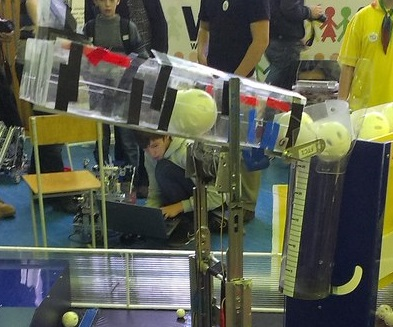
\includegraphics[scale=0.4]{days/13.12.14/images/01}}
			\caption{Крепление механизма опрокидывания ковша (на фото робот забрасывает мячи в 120-см корзину)}
		\end{minipage}
	\end{figure}
	
	\item В результате этого ковш не проходил между рейками и его пришлось подрезать.
	\begin{figure}[H]
		\begin{minipage}[h]{0.2\linewidth}
			\center  
		\end{minipage}
		\begin{minipage}[h]{0.6\linewidth}
			\center{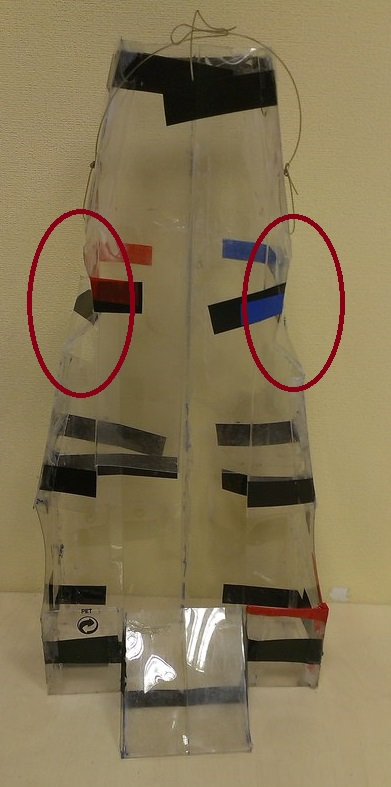
\includegraphics[scale=0.2]{days/13.12.14/images/02}}
			\caption{Ковш подрезан}
		\end{minipage}
	\end{figure}
	
	\item Все направляющие подъемника были тщательно смазаны для лучшего скольжения.
	
	\item Одна из двух стальных перекладин, установленных на подъемнике, оказывала слишком большое сопротивление движению ремня, вследствие чего ее пришлось заменить обратно на алюминиевую.
	
	\item Для улучшения качества захватывания маленьких мячей был установлен винт, притормаживающий лопасти. Таким образом лопасти сгибаются и в какой-то момент резко проворачиваются и за счет их упругости шарик "залетает" в ковш.
	\begin{figure}[H]
		\begin{minipage}[h]{0.2\linewidth}
			\center  
		\end{minipage}
		\begin{minipage}[h]{0.6\linewidth}
			\center{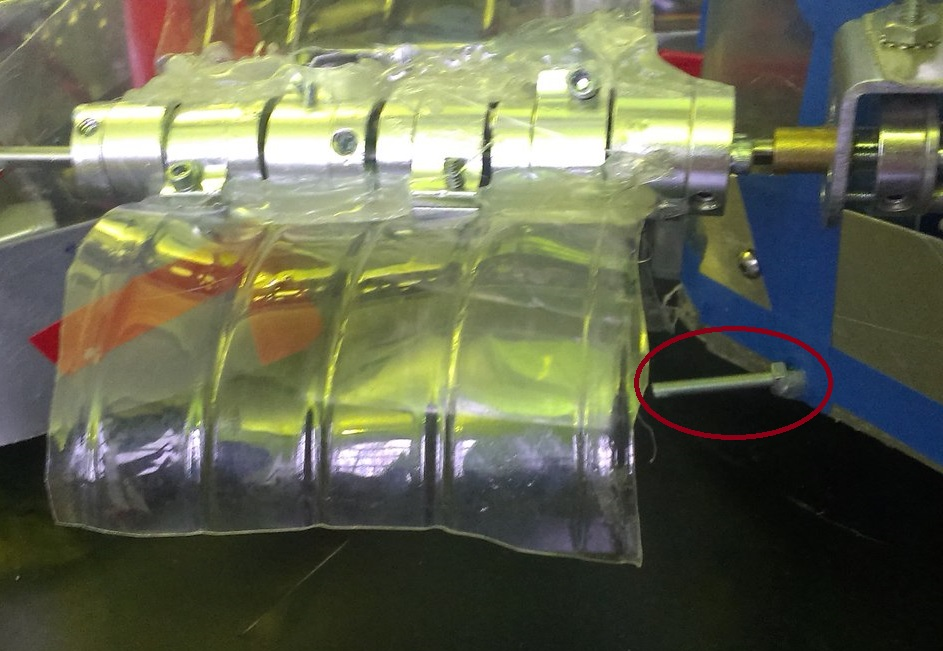
\includegraphics[scale=0.2]{days/13.12.14/images/03}}
			\caption{Винт}
		\end{minipage}
	\end{figure}
	
	\item На ковш был установлен механизм,напраляющий шары перпендикулярно поверхности земли.
	\begin{figure}[H]
		\begin{minipage}[h]{0.31\linewidth}
			\center{
\includegraphics[scale=0.22]{days/13.12.14/images/04}}
		\end{minipage}
		\hfill
		\begin{minipage}[h]{0.31\linewidth}
			\center{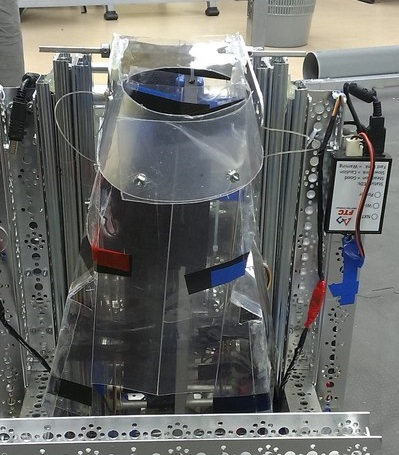
\includegraphics[scale=0.33]{days/13.12.14/images/05}}
		\end{minipage}
		\hfill
		\begin{minipage}[h]{0.31\linewidth}
			\center{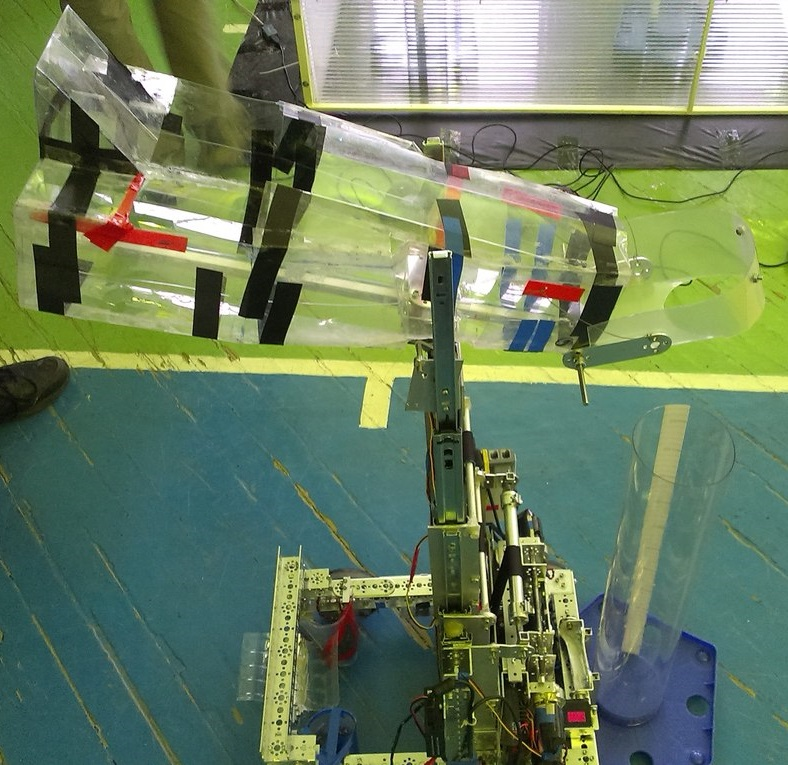
\includegraphics[scale=0.2]{days/13.12.14/images/06}}
		\end{minipage}
		\caption{Направляющая для шаров}
	\end{figure}
	
	\item Во время тренировок одну из поперечных осей на подъемнике вырвало из крепления. Это произошло из-за того, что отверстие, в которое она была вставлена было расположена слишком близко к краю пластины. Ось была переставлена.
	\begin{figure}[H]
		\begin{minipage}[h]{0.2\linewidth}
			\center  
		\end{minipage}
		\begin{minipage}[h]{0.6\linewidth}
			\center{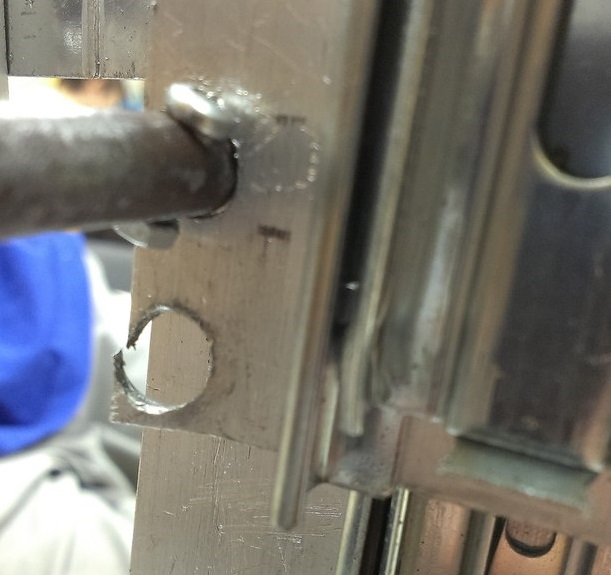
\includegraphics[scale=0.25]{days/13.12.14/images/07}}
			\caption{Вырванное крепление}
		\end{minipage}
	\end{figure}
	
	\item Программа автономного перида была корректирована под данные условия.
	
\end{enumerate}
\fillpage